\documentclass[tikz,border=2pt]{standalone}
\usepackage{pgfplots}
\usetikzlibrary{shapes.geometric, intersections}
\pgfplotsset{compat=1.7}

\begin{document}
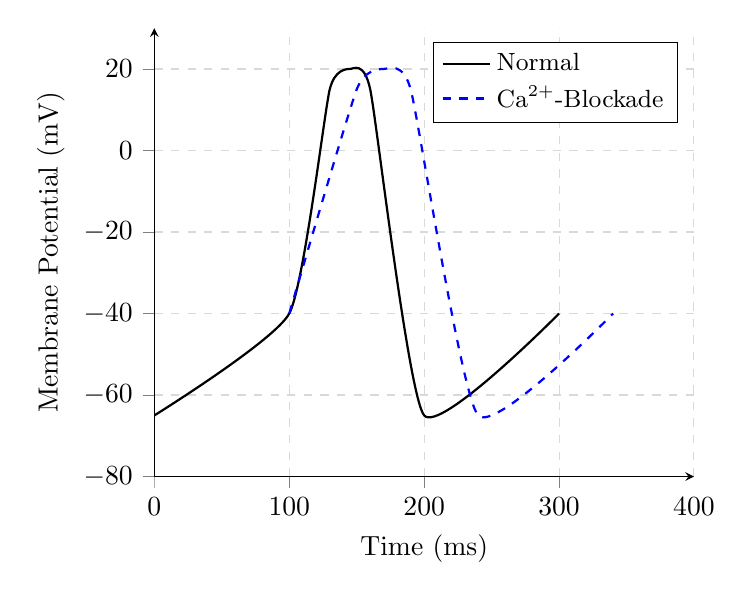
\begin{tikzpicture}

    \begin{axis}[
axis x line=bottom,
  axis y line=left,
	ymin = -80,
	ymax = 30,
	xmin = 0,
xmax = 400,
        grid = major,
        grid style={dashed, gray!30},
	 ylabel near ticks,
	xlabel near ticks,
        xlabel=Time (ms),
        ylabel=Membrane Potential (mV),
        tick align=outside,
        enlargelimits=false,
    legend pos=north east,
legend entries={Normal, Ca\textsuperscript{2+}-Blockade},
legend style={font=\small, cells={align=left}},
legend cell align={left}]

\draw[black, thick] plot[smooth,tension=0.3] coordinates { (axis cs: 0,-65) (axis cs: 100,-40) (axis cs: 130,15) (axis cs: 145,20) (axis cs: 160,15) (axis cs: 200,-65) (axis cs: 300,-40)};

\draw[blue, dashed, thick] plot[smooth,tension=0.3] coordinates {(axis cs: 100,-40) (axis cs: 150,15) (axis cs: 170,20) (axis cs: 190,15) (axis cs: 240,-65) (axis cs: 340,-40)};
  \addlegendimage{black, thick}
    \addlegendimage{blue,thick,dashed}


\end{axis}

\end{tikzpicture} 
\end{document}